\chapter{感知机(Perceptron)}


\section{超平面}

假设$\mathbb{R}^n$空间中的一个平面$S$,$S$上的一个法向量为
\begin{equation}
    \vec{n}=(\omega_1,\omega_2,\cdots,\omega_n)
\end{equation}

固定平面$S$的一个点$P_0=(x_0,x_1,\cdots,x_n)$,对于$S$上任意一个点$P=(x'_1,x'_2,\cdots,x'_n)$,构成一个向量
\begin{equation}
    \vec{x}=\Vec{PP_0}=(x'_1-x_1,x'_2-x_2,\cdots,x'_n-x_n)
\end{equation}

对于平面上任意一个向量,都与法向量垂直,因此平面方程表示为法向量和平面上任意一个向量的内积
\begin{eqnarray}
    \vec{n}\cdot \vec{x}=0
\end{eqnarray}

三维空间的平面称为平面,如果是任意的维度,广义的平面称为超平面。

\subsection*{实例}

对于平面上的点,因为都与超平面垂直,因此如果实例点落入超平面中,$\vec{n}\cdot \vec{x}=0$。对于位于超平面上方
的点,$PP_0$和法向量$n$之间的夹角
\begin{equation}
    \frac{PP_0\cdot n}{\Vert PP_0\Vert \Vert n\Vert}\leqslant 90^\circ
\end{equation}

因此在超平面上方的点都满足
\begin{equation}
    PP_0\cdot n\geqslant 0
\end{equation}

\begin{figure}
    \centering
    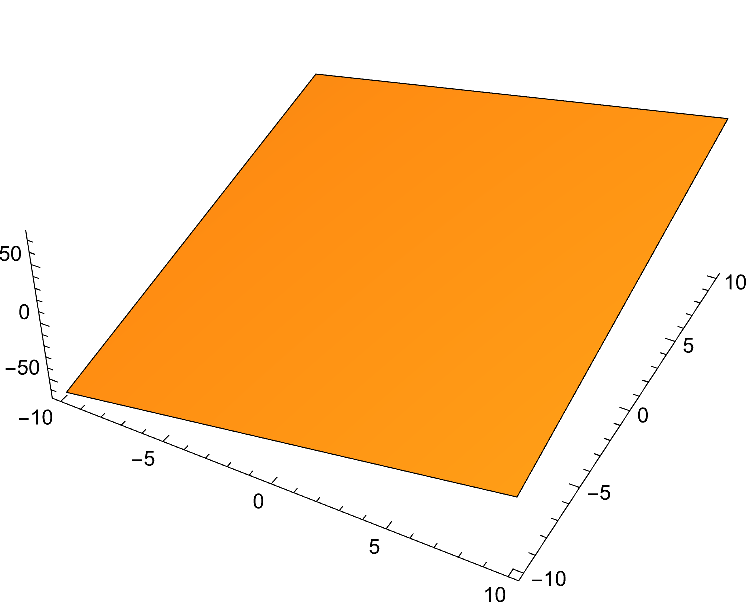
\includegraphics[scale=0.7]{figures/超平面.pdf}
    \caption{超平面}
\end{figure}

反之,超平面下方的点满足

\begin{equation}
    PP_0\cdot n\leqslant 0
\end{equation}

\section{模型}

\begin{define}
    (感知机) 假设输入空间(特征空间)$\mathcal{X}\subset \mathbb{R}^n$,输出空间是$\mathcal{y}=\{-1,+1\}$,
    输入$x\in \mathcal{X}$表示实例的特征向量,对应于输入空间(特征空间)的点;输出$y\in \mathcal{y}$表示实例的类别,
    由输入空间到输出空间的如下符号函数
    \begin{equation}
        f(x)=sign(\omega\cdot x+b)
    \end{equation}

    称为感知机。其中,$\omega$和$b$为感知机模型参数。
\end{define}


\section{数据集的线性可分性}

假设一个数据集
\begin{equation}
    T=\{(x_1,y_1),(x_2,y_2),\cdots,(x_n,y_n)\}
\end{equation}

如果存在一个超平面$\omega\cdot x+b=0$,使得数据集的正实例点和负实例点完全正确地划分到超平面的两侧处,即对所有的$y_i=+1$
的实例$i$,有
\begin{equation}
    \omega\cdot x_i+b>0
\end{equation}

对所有的$y_i=-1$的实例$i$,
\begin{equation}
    \omega\cdot x_i+b<0
\end{equation}


则$T$被称为线性可分的数据集。


\section{损失函数}

\subsection*{实例点误分类的判别关系}

根据输入空间到输出空间的映射方式,误分类的实例点应该满足下面的关系。
\begin{equation}
    -y_i(\omega\cdot x_i+b)>0
\end{equation}

\subsection*{感知机的损失函数}

损失函数一个自然选择是误分类点的总数,但是这样损失函数就不是参数$\omega$和$b$。但是可以
考虑:如果所有误分类点距离超平面的距离为0,则这是一次完美的分割。

输入空间$R^n$中任意一点$x$到超平面$S$到距离为
\begin{equation}
    \frac{1}{\Vert \omega\Vert}|\omega\cdot x+b|
\end{equation}

对于误分类的数据来说,距离为

\begin{equation}
    \frac{1}{\Vert \omega\Vert}y_i(\omega\cdot x+b)
\end{equation}\footnote{因为$y_i$只能去+1和-1,因此可以把绝对值符号去掉}

所有误分类点到超平面$S$到总距离为
\begin{equation}
    L=-\frac{1}{\Vert \omega\Vert}\sum_{x_i\in M}^{n}y_i(\omega\cdot x_i+b)
\end{equation}

\section{感知机学习算法}

给定一个训练数据集
\begin{eqnarray}
    T=\{(x_1,y_1),(x_2,y_2),\cdots,(x_N,y_N)\}
\end{eqnarray}

其中$x_i\in \mathcal{X}=R^n$,$y_i\in\mathcal{Y}=\{-1,1\}$,$i=1,2,\cdots,N$,求参数$\omega$、$b$
使得损失函数最小化
\begin{equation}
    \min\limits_{\omega,b}L(\omega,b)=-\sum_{x_i\in M}y_i(\omega\cdot x_i+b)
\end{equation}

其中$M$是误分类点集合。

\subsection*{原始形式}

\begin{framed}
输入:训练数据集$T$;设定学习率$\eta\ (0<\eta\leqslant 1)$;

输出:$\omega,b$;$f(x)=sign(\omega\cdot x+b)$;

\begin{enumerate}[itemindent=1em]
    \item 选定初值$\omega_0,b_0$;
    \item 在训练集中选取数据$(x_i,y_i)$;
    \item 如果$y_i(\omega\cdot x_i+b)\leqslant 0$,更新权重
    \begin{equation}
        \begin{aligned}
            & \omega\leftarrow \omega+\eta y_ix_i\\
            & b \leftarrow b+\eta y_i
        \end{aligned}
    \end{equation}
    \item 跳转至2,直到没有误分类点。
\end{enumerate}
\end{framed}

\subsection*{对偶形式}

\begin{framed}
输入:训练数据集$T$;设定学习率$\eta\ (0<\eta\leqslant 1)$;

输出:$\alpha,b$;$f(x)=sign(\sum_{j=1}^{N}\alpha_jy_jx_j\cdot x+b)$,其中$\alpha=(\alpha_1,\alpha_2,\cdots,\alpha_N)^T$;

\begin{enumerate}[itemindent=1em]
    \item $\alpha \leftarrow 0$,$b\leftarrow 0$;
    \item 训练集上选取数据$(x_i,y_i)$;
    \item 如果$y_i(\sum_{j=1}^{N}\alpha_jy_jx_j\cdot x_i+b)\leqslant 0$
    \begin{equation}
        \begin{aligned}
            & \alpha_i\leftarrow \alpha_i+\eta\\
            & b\leftarrow b+\eta y_i
        \end{aligned}
    \end{equation}

    \item 跳转到2直到没有误分类点数据。
\end{enumerate}
    
\end{framed}

对偶形式的基本想法是,将$\omega$和$b$表示为实例$x_i$和$y_i$的线性组合的形式,通过
求解其系数而求得$\omega$和$b$。不失一般性,在原始形式算法中假设初始值均为0,对误分类点
$(x_i,y_i)$通过
\begin{eqnarray}
    \begin{aligned}
        & \omega \leftarrow \omega +\eta y_i x_i\\
        & b\leftarrow b+\eta y_i
    \end{aligned}
\end{eqnarray}

逐步修改$\omega$和$b$,修改$n$次的$\omega$和$b$增量为$\alpha_iy_ix_i$和$\alpha_iy_i$。
这里$\alpha_i=n_i\eta$。这样,从学习过程不难看出,最后学习到的$\omega,b$可以分别表示为
\begin{equation}
    \omega = \sum_{i=1}^{N} \alpha_iy_ix_i
\end{equation}

\begin{equation}
    b=\sum_{i=1}^{N} \alpha_iy_i
\end{equation}

这里$\alpha_1\geqslant 1,\ i=1,2,\cdots,N$,当$\eta=1$时,表示第$i$个实例点由于误分类而进行
更新的次数。实例点更新次数越多,意味着它距离超平面越近,也就越难正确分类。这样的实例对学习结果影响最大。

\section{感知机收敛定理}

\begin{theorem}
    (Novikoff) 设训练数据集$T=\{(x_1,y_1),(x_2,y_2),\cdots,(x_N,y_N)\}$是线性可分
    的数据集,其中$x_i\in \mathcal{X}=R^n$,$y_i\in \mathcal{Y}={-1,+1}$,$i=1,2,\cdots,N$,
    则
    \begin{enumerate}[itemindent=2em]
        \item 存在满足条件$\Vert \hat{\omega}_{opt}=1\Vert$的超平面$\hat{\omega}_{opt}\cdot \hat{x}=\omega_{opt}\cdot x+b_{opt}=0$将
        训练数据集完全正确分开;且存在$\gamma>0$,对于所有$i=1,2,\cdots,N$
        \begin{equation}
            y_i(\hat{\omega}_{opt}\cdot\hat{x})=y_i(\omega_{opt}\cdot x_i+b_{opt})\geqslant \gamma
        \end{equation}

        \item 令$R=\max\limits_{1\leqslant i\leqslant N}\Vert \hat{x}_i \Vert$,则感知机算法在训练数据集上的误分类次数$k$满足不等式
        \begin{eqnarray}
            k\leqslant (\frac{R}{\gamma})^2
        \end{eqnarray}
    \end{enumerate}
\end{theorem}

\textbf{proof. } 首先证明第一点:

由于训练集数据是线性可分的,按照定义,存在超平面可以将数据集完全正确分开,取此超平面为
\begin{equation}
    \hat{\omega}_{opt}\cdot \hat{x}=\omega_{opt}\cdot+b_{opt}=0
\end{equation}

由于等式右边等于0,所以总可以取$\Vert \hat{\omega}\Vert=1$。对于有限的$i=1,2,\cdots,N$,正确分类下有
\begin{equation}
    y_i(\hat{\omega}_{opt}\cdot \hat{x}_i)=y_i(\omega_{opt}\cdot x_i+b_{opt})>0
\end{equation}

所以$0$是序列$\{ y_i(\hat{\omega}_{opt}\cdot \hat{x}_i)\}$的一个下界,假设序列的下确界
\begin{equation}
    \gamma=\inf\limits_{i}\{y_i(\omega_opt\cdot x_i+b_{opt})\}
\end{equation}

使得
\begin{equation}
    y_i(\hat{\omega}_{opt}\cdot \hat{x}_i)=y_i(\omega_{opt}\cdot x_i+b_{opt})\geqslant \gamma \geqslant 0
\end{equation}

下面证明第二点:

训练点为$x_i$,标签为$y_i$。假设$\hat{\omega}_{opt}=0$开始,如果实例被误分类,则更新权重。令$\hat{\omega}_{k-1}$是
第$k$个误分类实例之前的扩充权重向量,即
\begin{equation}
    \hat{\omega}_{k-1}=(\omega_{k-1}^T,b_{k-1})^T
\end{equation}

如果第$k$个实例点是误分类点,则
\begin{equation}
    y_i(\hat{\omega}_{k-1}\cdot \hat{x}_i)=y_i(\omega_{k-1}\cdot x_i+b_{k-1})\leqslant 0
\end{equation}

在误分类的时候更新权重
\begin{equation}
    \begin{aligned}
        & \omega_k\leftarrow \omega_{k-1}+\eta y_ix_i\\
        & b_k \leftarrow b_{k-1}+\eta y_i
    \end{aligned}
\end{equation}

即
\begin{equation}
    \hat{\omega}_{k}=\hat{\omega}_{k-1}+\eta y_i\hat{x}_i
    \label{eq1.31}
\end{equation}

利用两个不等式,这两个不等式将在后续的引理中证明。
\begin{equation}
    \hat{\omega}_k\cdot \hat{\omega}_{opt} \geqslant k\eta \gamma
\end{equation}
\begin{equation}
    \Vert \hat{\omega}_k\Vert^2\leqslant k\eta^2R^2
\end{equation}

代入方程(\ref{eq1.31}),得到
\begin{equation}
    \begin{aligned}
        & k\eta \gamma \leqslant \hat{\omega}_k\cdot \hat{\omega}_{opt}\leqslant \Vert\hat{\omega}_k\Vert 
        \Vert\hat{\omega}_{opt}\Vert \leqslant \sqrt{k}\eta R\\
        & k^2\gamma^2\leqslant kR^2
    \end{aligned}
\end{equation}

于是
\begin{equation}
    k\leqslant (\frac{R}{\gamma})^2
\end{equation}









